\section{特性：有效的语义异构体}

我们接下来分析为何表层蒸馏会失败：即便概念“原子”相同，不同的键连接方式也会形成完全不同的推理链——我们称其为\textbf{语义异构体}。形式上，若 \(\mathcal{D}\) 的一个语义异构体 \(\mathcal{D}'\) 的转移分布 \((P_{\mathcal{D}'}, \pi_{\mathcal{D}'})\) 与 \((P_{\mathcal{D}}, \pi_{\mathcal{D}})\) 在某个散度度量 \(D(\cdot\,\|\,\cdot)\) 下足够接近，则 \(\mathcal{D}'\) 可视作 \(\mathcal{D}\) 的异构体。下面我们分析它们如何形成、被学习，以及在 Long CoT 中何时失效。

\subsection{语义异构体的键结构是 Long CoT 学习的关键}

\paragraph{\textbf{结构良好的语义异构体可以有效促进 Long CoT 学习。}}
我们构造了一份由强推理模型蒸馏得到的长链数据集，用来评估这类异构体是否能提升 Long CoT 学习。表~\ref{tab:distill_result} 显示，蒸馏自不同“异构体”数据集的模型都获得了稳定收益，其分布相关性约为 0.9。这说明在一定范围内，推理关键分布存在多个有效“同素异形体”。\vspace{-8pt}



\paragraph{\textbf{模型存在多种有效的语义异构体，但微小差异即可显著影响结果。}}
表~\ref{tab:distill_result} 显示，R1 与 OSS 的链结构相关性可达 0.95，但部分模型在 R1 链上的表现仍下降 10\% 以上。这表明存在多种近似最优却脆弱的语义异构体，只要分布稍有变化，性能就会大幅下跌。\vspace{-8pt}

\begin{wrapfigure}{r}{0.32\textwidth}
    \centering
    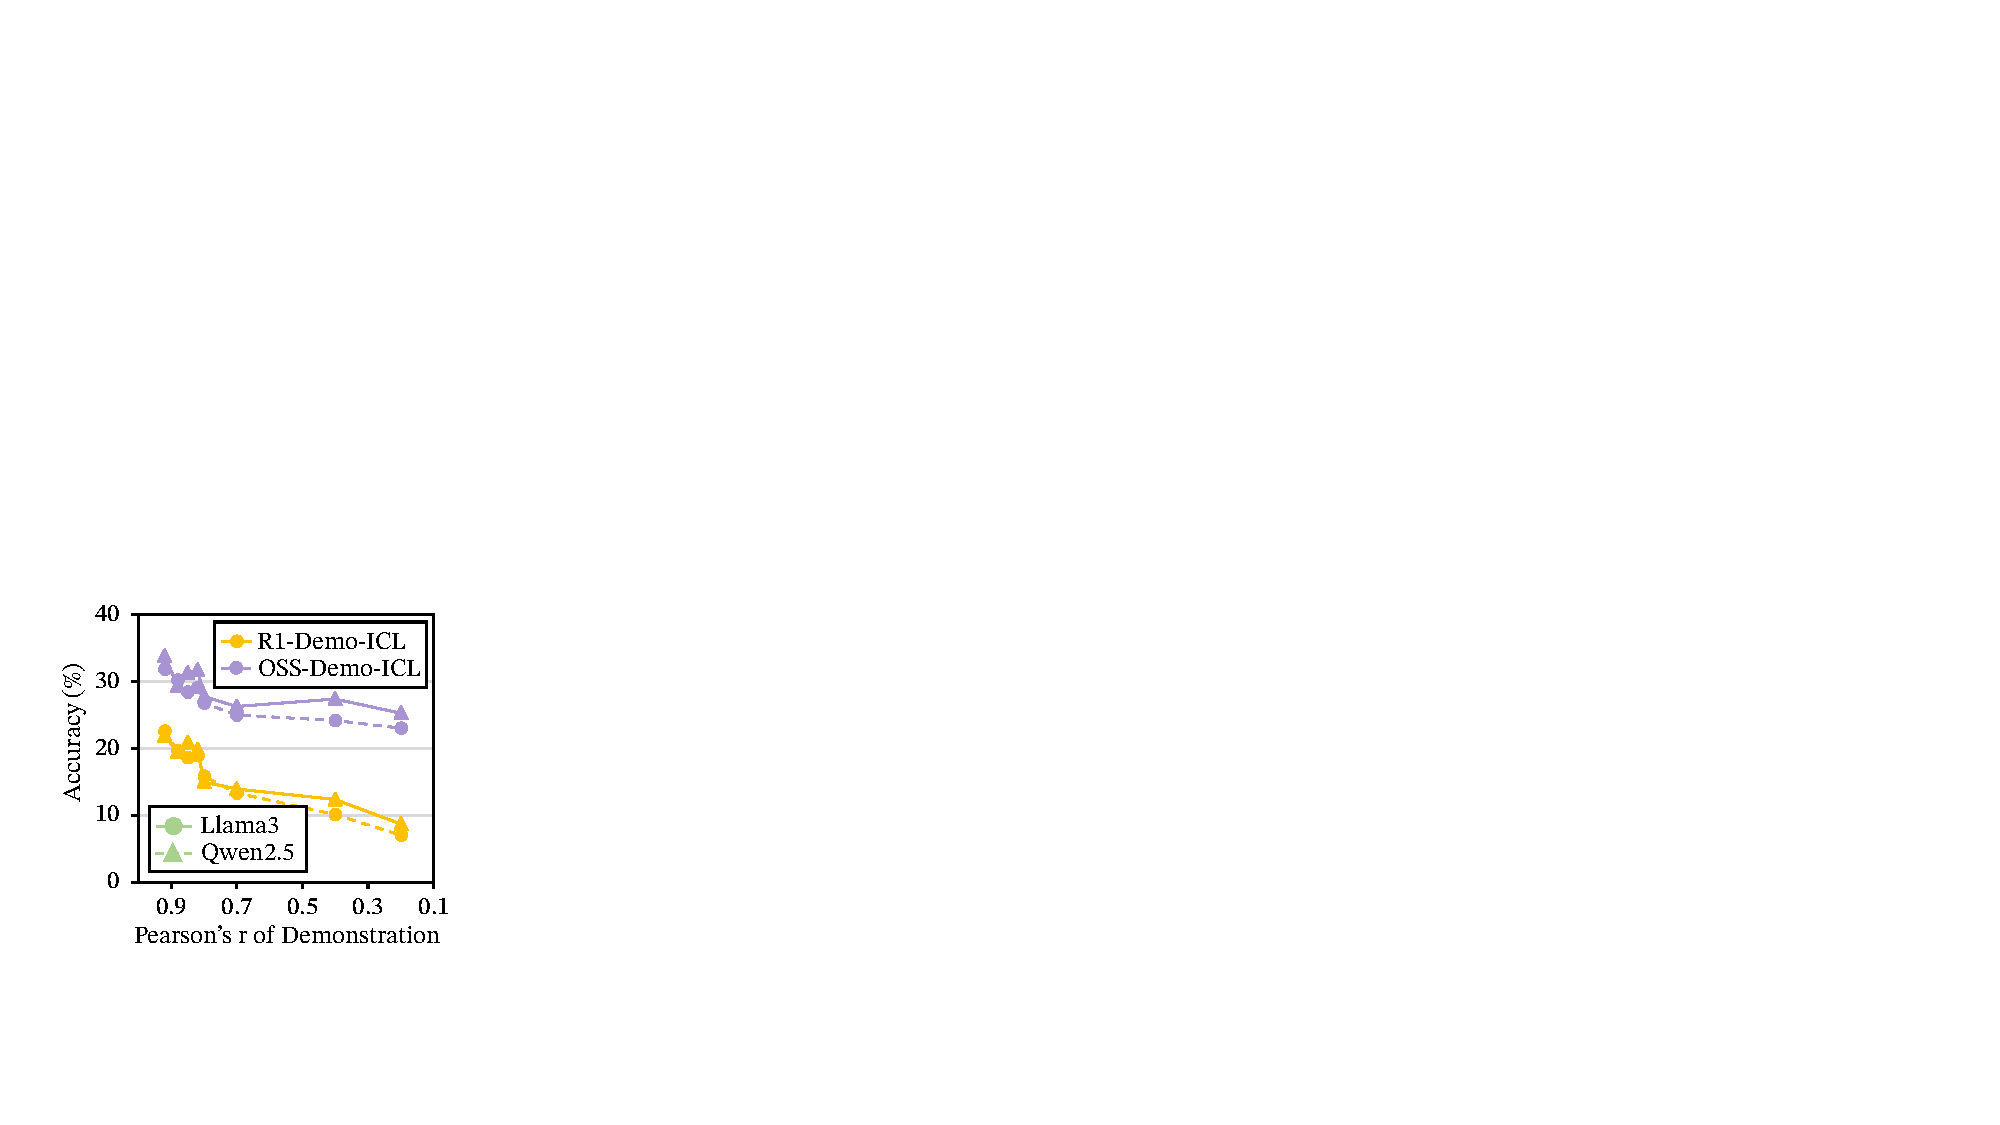
\includegraphics[width=0.30\textwidth]{figures/icl.pdf}
    \caption{LLama-3.1-8B-Instruction 在三种 ICL 蒸馏设置下的表现（教师为 ICL 增强的 Qwen2.5-32B）。}
    \vspace{-20pt}
    \label{fig:icl}
\end{wrapfigure}
\paragraph{\textbf{仿真有效语义异构体结构是 ICL 蒸馏成功的关键。}}
我们考察 Qwen2.5-32B-Instruct 的三种 ICL 设置：随机挑选示例、匹配目标推理关键分布（相关约 0.9）、明显不匹配的分布（相关 $< 0.8$）。图~\ref{fig:icl} 显示，只有当示例被构造成与目标分布高度一致时，模型才能获得显著收益。这说明 ICL 蒸馏的核心在于模拟目标结构的“同素异形体”。



\begin{figure*}[t]
    \centering
    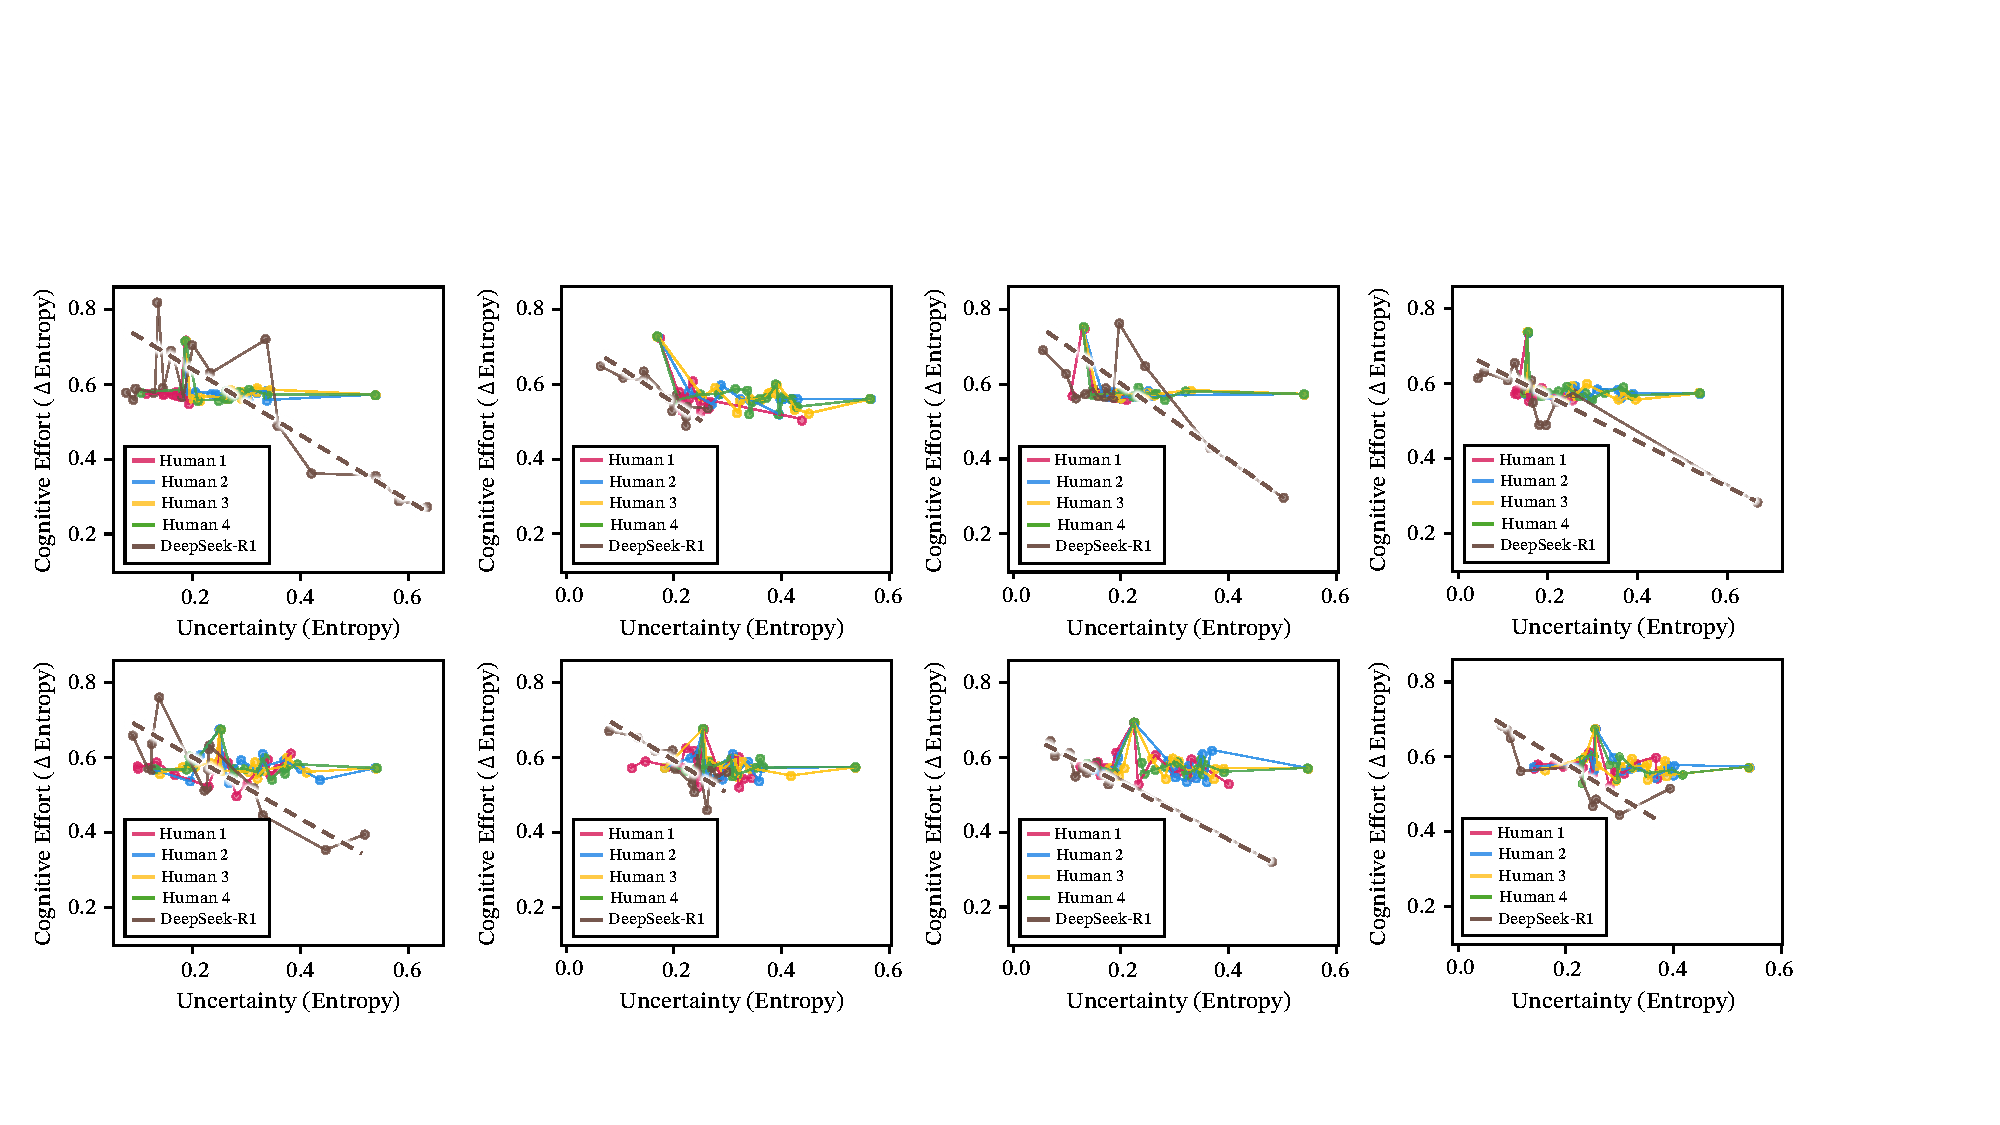
\includegraphics[width=\textwidth]{figures/effect-full.pdf}
    \caption{人类与推理模型在信息流上的差异分析。}
    \label{fig:effect}
\end{figure*}


\begin{figure*}[t]
    \centering
    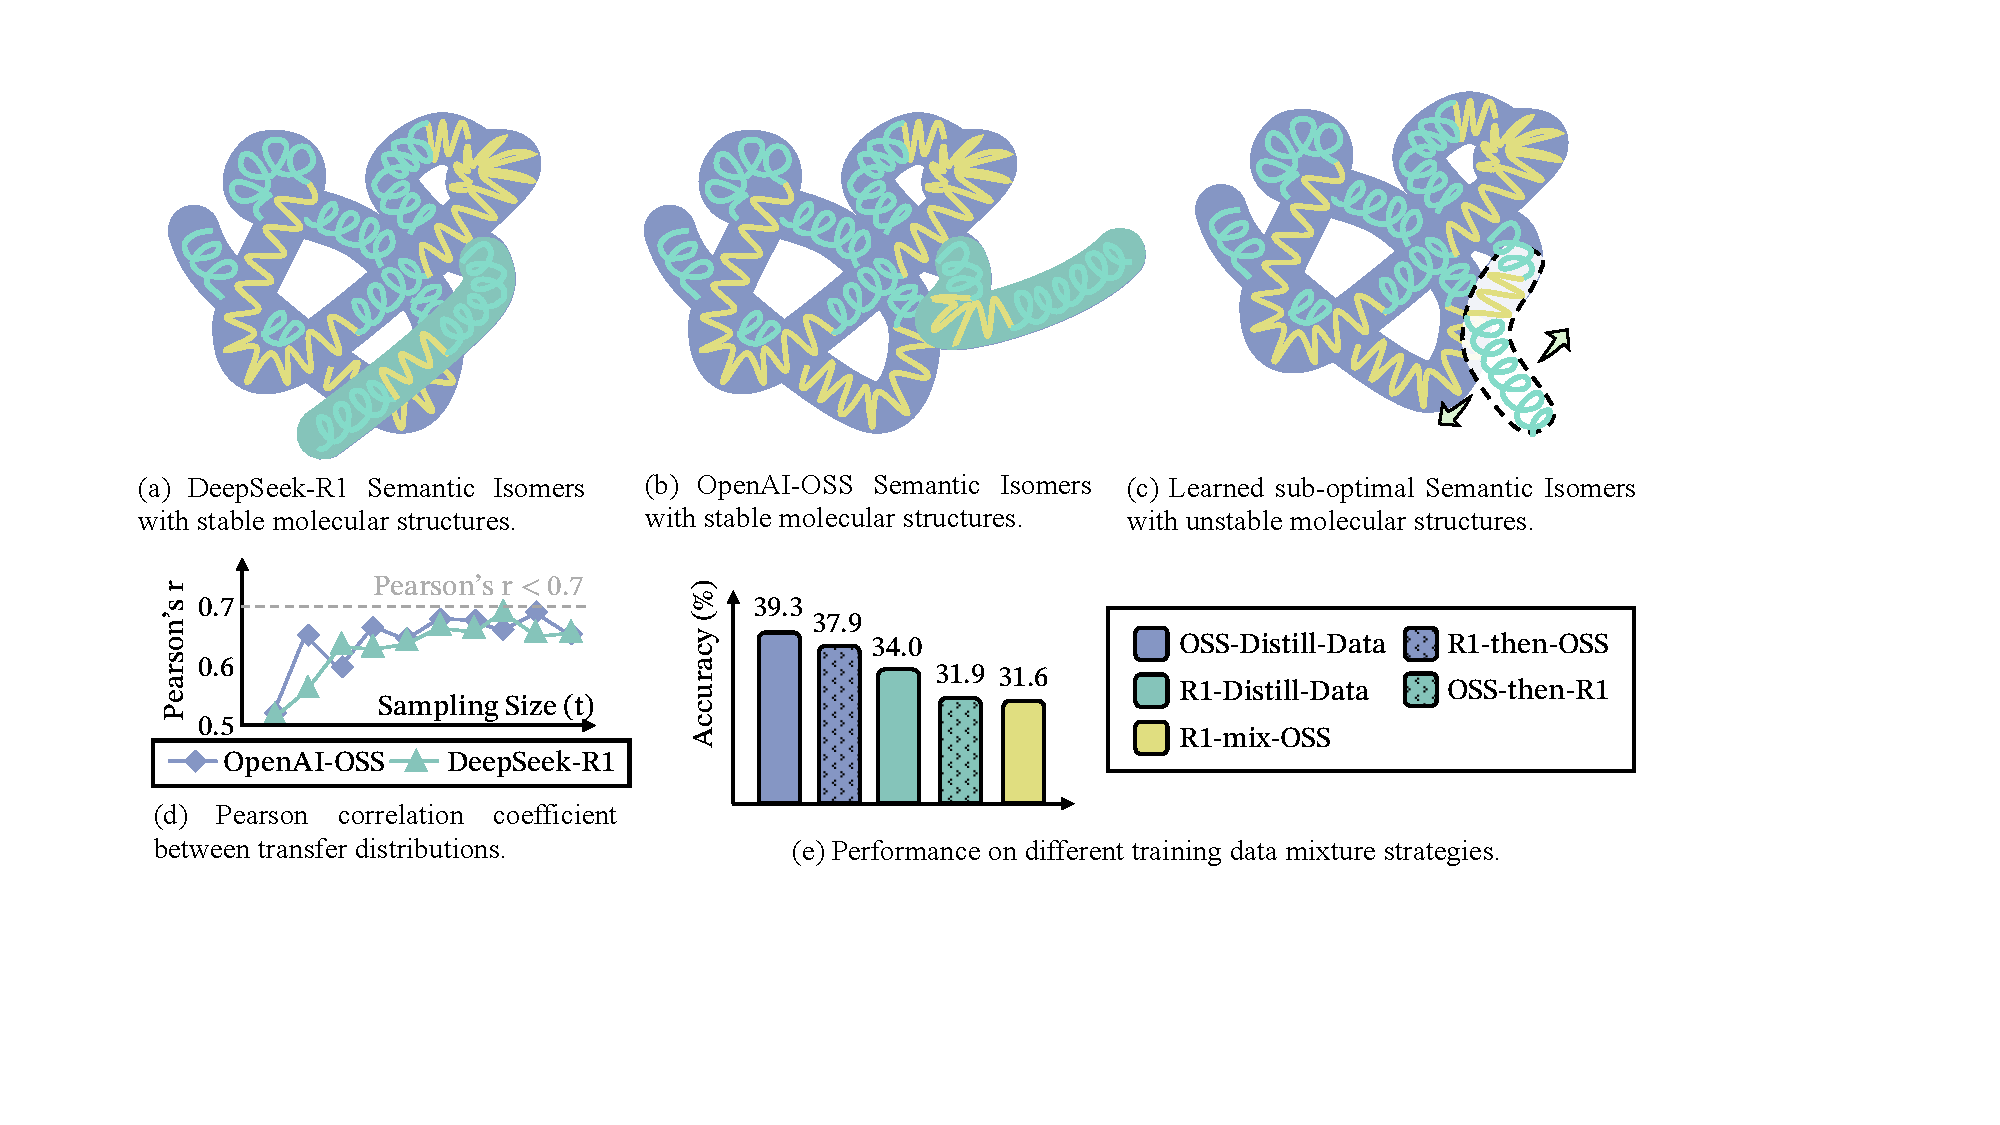
\includegraphics[width=0.98\textwidth]{figures/conflict.pdf}
    \caption{两种稳定分子结构之间的“冲突学习”。}
    
    \label{fig:conflict}
\end{figure*}
\subsubsection{并非所有键都有效}

为澄清语义异构体的本质，我们探究哪些键分布能够构成有效推理结构。我们的假设是：功能可行性取决于特定的键分布——即便概念节点一致，不兼容的结构也会干扰信息交换。例如，探索键过多会导致推理破碎，而过度强调深层推理会使链条僵化，难以适应新输入。细节见附录~\ref{append:information}。\vspace{-8pt}


\paragraph{\textbf{有效的推理键分布影响推理动态中的信息散度速度。}}
我们在信息相位空间中比较了 R1 模型与人类认知~\cite{chen2025universal} 的推理动态。LLM 的更新本质上是在奖励最大化下减小熵，而人类推理还受语义一致性与社会反馈约束。因此，机器推理通过累计梯度更新收敛，而人类则依赖自我监控与社会校准。
如图~\ref{fig:effect} 所示，我们在逻辑推理任务中追踪了长链推理的信息演化。人类的前进收益几乎均匀（81.3\% 的案例变化小于 0.1），对应相位空间中的近零斜率；而 R1 模型呈加速增益（76.1\% 的案例变化大于 0.1），从高熵状态迅速收敛。这说明 R1 与人类在时间维度上整合信息的方式根本不同。\vspace{-8pt}


\paragraph{\textbf{有效推理键引发元认知振荡并促进对齐。}}
我们发现差异的核心在于 LLM 的“元认知振荡”：响应在高熵的发散探索（斜率 $>0.6$、熵增 $>0.05$）与稳定的收敛验证之间交替，而人类则更接近均匀熵轨迹。图~\ref{fig:effect} 的案例表明，R1 模型利用自我反思来对抗不确定性并修正推理路径。我们推测，只要让训练目标与这些行为结构分布对齐，就能缩小机器与人类推理动态之间的差距。

\subsection{两种稳定结构之间的冲突}

理解不同推理结构如何交互，有助于揭示复杂认知系统的基本限制。图~\ref{fig:conflict}(a–c) 表明，硬性融合两个稳定的分子异构体会破坏骨架；同理，把不兼容的推理框架拼接在一起会打破全局连贯性。\vspace{-8pt}

\paragraph{\textbf{同时学习两种异构体会导致结构混乱。}}
如图~\ref{fig:conflict}(d)，我们让模型同时激活来自 DeepSeek-R1 与 OpenAI-OSS 的两条高度相关（$r \approx 0.9$）推理链。尽管它们表面接近，并行激活会阻止模型收敛到单一稳定模式：分子键分布在样本间剧烈波动，偏离 R1 或 OSS 的特征。相应地，混合模型的自相关度无法超过 0.8。\vspace{-8pt}

\paragraph{\textbf{结构混乱会显著拉低性能。}}
图~\ref{fig:conflict}(e) 显示，相比任何单一链路，联合激活都会导致显著的性能下降。这个现象说明，决定异构体能否共存的并非统计相关性，而是结构兼容性。干涉模式表明，底层认知架构是刚性的；若不精心对齐，盲目融合只会产出支离破碎、低价值的输出。


\begin{TakeawayBox}{结论 3}
\begin{itemize}[leftmargin=16pt, itemsep=0pt, topsep=0pt]
    \item 只要推理关键分布足够接近，结构良好的异构体就能有效发挥作用；但细微的结构漂移会引发脆弱性和精度崩塌；
    \item 把不兼容的推理结构强行并用，会造成结构混乱，从而破坏连贯性并显著降低性能，这证明单纯的统计相似性不足以保障兼容性。
\end{itemize} 
\end{TakeawayBox}
